% !TeX program = XeLaTeX


\documentclass[12pt,a4paper]{article}\usepackage[]{graphicx}\usepackage[]{color}
%% maxwidth is the original width if it is less than linewidth
%% otherwise use linewidth (to make sure the graphics do not exceed the margin)
\makeatletter
\def\maxwidth{ %
  \ifdim\Gin@nat@width>\linewidth
    \linewidth
  \else
    \Gin@nat@width
  \fi
}
\makeatother

\definecolor{fgcolor}{rgb}{0.345, 0.345, 0.345}
\newcommand{\hlnum}[1]{\textcolor[rgb]{0.686,0.059,0.569}{#1}}%
\newcommand{\hlstr}[1]{\textcolor[rgb]{0.192,0.494,0.8}{#1}}%
\newcommand{\hlcom}[1]{\textcolor[rgb]{0.678,0.584,0.686}{\textit{#1}}}%
\newcommand{\hlopt}[1]{\textcolor[rgb]{0,0,0}{#1}}%
\newcommand{\hlstd}[1]{\textcolor[rgb]{0.345,0.345,0.345}{#1}}%
\newcommand{\hlkwa}[1]{\textcolor[rgb]{0.161,0.373,0.58}{\textbf{#1}}}%
\newcommand{\hlkwb}[1]{\textcolor[rgb]{0.69,0.353,0.396}{#1}}%
\newcommand{\hlkwc}[1]{\textcolor[rgb]{0.333,0.667,0.333}{#1}}%
\newcommand{\hlkwd}[1]{\textcolor[rgb]{0.737,0.353,0.396}{\textbf{#1}}}%
\let\hlipl\hlkwb

\usepackage{framed}
\makeatletter
\newenvironment{kframe}{%
 \def\at@end@of@kframe{}%
 \ifinner\ifhmode%
  \def\at@end@of@kframe{\end{minipage}}%
  \begin{minipage}{\columnwidth}%
 \fi\fi%
 \def\FrameCommand##1{\hskip\@totalleftmargin \hskip-\fboxsep
 \colorbox{shadecolor}{##1}\hskip-\fboxsep
     % There is no \\@totalrightmargin, so:
     \hskip-\linewidth \hskip-\@totalleftmargin \hskip\columnwidth}%
 \MakeFramed {\advance\hsize-\width
   \@totalleftmargin\z@ \linewidth\hsize
   \@setminipage}}%
 {\par\unskip\endMakeFramed%
 \at@end@of@kframe}
\makeatother

\definecolor{shadecolor}{rgb}{.97, .97, .97}
\definecolor{messagecolor}{rgb}{0, 0, 0}
\definecolor{warningcolor}{rgb}{1, 0, 1}
\definecolor{errorcolor}{rgb}{1, 0, 0}
\newenvironment{knitrout}{}{} % an empty environment to be redefined in TeX

\usepackage{alltt}
\usepackage{amsmath,amssymb,amsthm}
\usepackage{setspace}
%\usepackage[semicolon,sort]{natbib}
\usepackage[backend=biber,citestyle=authoryear-comp,natbib=true,sorting=nyt,sortcites=true,maxnames=10,giveninits=false,uniquename=false,doi=false,url=false,isbn=false]{biblatex} % Numbered citations
%\usepackage[backend=biber,citestyle=authoryear-comp,natbib=true,sorting=nyt,sortcites=true,maxnames=10,firstinits=false,uniquename=false]{biblatex}
\addbibresource{grouprec.bib}
\usepackage{geometry}
\usepackage{verbatim}
\usepackage{tabularx}
\usepackage[usenames]{xcolor}
\usepackage[right,official]{eurosym}
\usepackage{threeparttable,rotating,floatrow}
\floatsetup[table]{style=Plaintop}
\usepackage[bottom]{footmisc}
\usepackage{graphicx}\graphicspath{{../Data/}}
\usepackage[labelfont=sf,textfont=sf,bf]{caption}
\usepackage{subcaption}
\usepackage{ragged2e}
\usepackage{booktabs,multirow,array}
\usepackage[hidelinks,pdfstartview=]{hyperref}
\usepackage{changepage} % needed for the appendix

%\usepackage[nolists]{endfloat}
%\usepackage[affil-it]{authblk}
%\renewcommand\Authfont{\sffamily}
%\renewcommand\Affilfont{\sffamily\small\it}
%\setlength{\affilsep}{0.5em}
\usepackage{xltxtra,fontspec,xunicode}
\defaultfontfeatures{Mapping=tex-text}
\setsansfont{TeX Gyre Heros}
\setromanfont{Charis SIL}
\setromanfont{Heuristica}

\onehalfspacing

\usepackage{siunitx}
\newcolumntype{x}[1]{>{\centering\arraybackslash}m{#1}}%
\newcommand{\specialcell}[2][c]{%
  \begin{tabular}[#1]{@{}c@{}}#2\end{tabular}}

\makeatletter
%\def\@seccntformat#1{}
%%% Change section and subsection style
\renewcommand\section{\@startsection {section}{1}{\z@}%
{-3.5ex \@plus -1ex \@minus -.2ex}%
{2.3ex \@plus.2ex}%
{\bf\sffamily\Large}}
\renewcommand\subsection{\@startsection {subsection}{1}{\z@}%
{-3.5ex \@plus -1ex \@minus -.2ex}%
{2.3ex \@plus.2ex}%
{\it\large}}
\makeatother

%%% Define subhyps

\makeatletter
\newcounter{subhyp}
\let\savedc@hyp\c@hyp
\newenvironment{subhyp}
 {%
  \setcounter{subhyp}{0}%
  \stepcounter{hyp}%
  \edef\saved@hyp{\thehyp}% Save the current value of hyp
  \let\c@hyp\c@subhyp     % Now hyp is subhyp
  \renewcommand{\thehyp}{\saved@hyp\alph{hyp}}%
 }
 {}
\newcommand{\normhyp}{%
  \let\c@hyp\savedc@hyp % revert to the old one
  \renewcommand\thehyp{\arabic{hyp}}%
}
\makeatother

\renewcommand{\abstractname}{\bf\sffamily Abstract}

\newtheorem{hyp}{Hypothesis}
\newtheorem{res}{Result}

\title{\bf\sffamily Humans reciprocate intentional harm by discriminating against group peers}
%\author{\textsc{Authors undisclosed}}
\author{David Hugh-Jones\thanks{School of Economics, University of East Anglia. E-mail: d.hugh-jones@uea.ac.uk.} \and Itay Ron\thanks{E-mail: itayron@gmail.com} \and Ro'i Zultan\thanks{Corresponding author, Department of Economics, Ben-Gurion University of the Negev. E-mail: zultan@bgu.ac.il.}}

\date{}%\sffamily \small This version: \today.}

%\textbf{Preliminary version, please do not distribute.}}

\def\figwidth{\textwidth}
\IfFileExists{upquote.sty}{\usepackage{upquote}}{}
\begin{document}
%\SweaveOpts{concordance=TRUE}
\maketitle

\begin{abstract}
The evolution of human intergroup conflict is a social science puzzle. 
Motivated by cycles of intergroup revenge in real-world conflicts, we experimentally
test the hypothesis that humans practice group-based reciprocity: if someone
harms or helps them, they harm or help other members of that person's group.
Subjects played a trust game, then allocated money between other people. Senders
whose partners returned more in the trust game gave more to that partner's group
members. The effect was about half as large as the effect of direct reciprocity.
Receivers' allocations to group members were not affected by their partners’ 
play in the trust game, suggesting that group reciprocity was only triggered when the
partner's intentions were unequivocal. We show conditions under which group 
reciprocity can evolve, and discuss its place in conflict among early humans.
\end{abstract}

\emph{Keywords:} Upstream reciprocity, group identity, intergroup conflict.

Word count: 3129

%Q\section*{Significance statement}

%Sometimes humans take revenge, not on the person who harmed them, but on other people from that person's group. This can lead to intergroup conflict and violence. We ran a laboratory experiment showing that this happens. We found that humans only take revenge on groups when the original person's act was deliberate and unequivocal. Laboratory experiments like these can help us to understand the psychology behind intergroup revenge.

\newpage

\section{Introduction}

Human society is organized in groups, including families, clans, firms and nations. This
structure is reflected in individual behaviour and cognition. Humans identify
with their ingroup and are altruistic and prosocial towards ingroup members;
towards outgroup members, they display stereotyping and prejudice
\citep{tajfel1979integrative,yamagishi2000thegroup,balliet2014ingroup,DeDreu2014,chen2009group,chen2011potential}.
Group structure provides the backdrop for intergroup conflict---from economic
and political competition to inter-ethnic violence and war---which is pervasive
in the species \citep{world_bank_world_2011}.

Intergroup conflicts often follow a tit-for-tat logic, in which one group's
violence leads to revenge from the other side
\citep{horowitz2001thedeadly,horowitz1985ethnicgroups,chagnon1988lifehistories,haushofer_both_2010,shayo2010judicial}.
This suggests that humans practice intergroup \emph{reciprocity}. Reciprocity is
a well-known mechanism that may underlie the evolution of cooperation
\citep{nowak2006five,nowak2012evolving}. While in direct reciprocity,
individuals help those who have helped them in the past (and similarly for
harm), in indirect reciprocity, individuals help or harm other people than those
who have helped them.  Indirect reciprocity comes in two flavours:
\emph{downstream} reciprocity follows the maxim `do unto thy neighbour as they
have done to others', whereas \emph{upstream} reciprocity follows the maxim `do
unto thy neighbour as others have done unto you'. 
%There is evidence for group-based downstream reciprocity: individuals punish norm violators more if these harm a member of their own group \citep{bernhard2006group,bernhard2006parochial}. 

In this paper we examine
group-based upstream reciprocity, or \emph{group reciprocity}. That is, an
individual who is harmed (helped) by a member of an outgroup becomes more likely
to harm (help) others from that group.  Whereas group-based downstream
reciprocity \citep{bernhard2006group,bernhard2006parochial} follows the maxim
`do unto others as they have done to members of \emph{my} tribe', group-based
upstream reciprocity follows the maxim `do unto others as members of
\emph{their} tribe have done to me' (Figure~\ref{fig:illustration}).

\begin{figure}
	\begin{center}
        \begin{subfigure}[b]{0.4\textwidth}
		  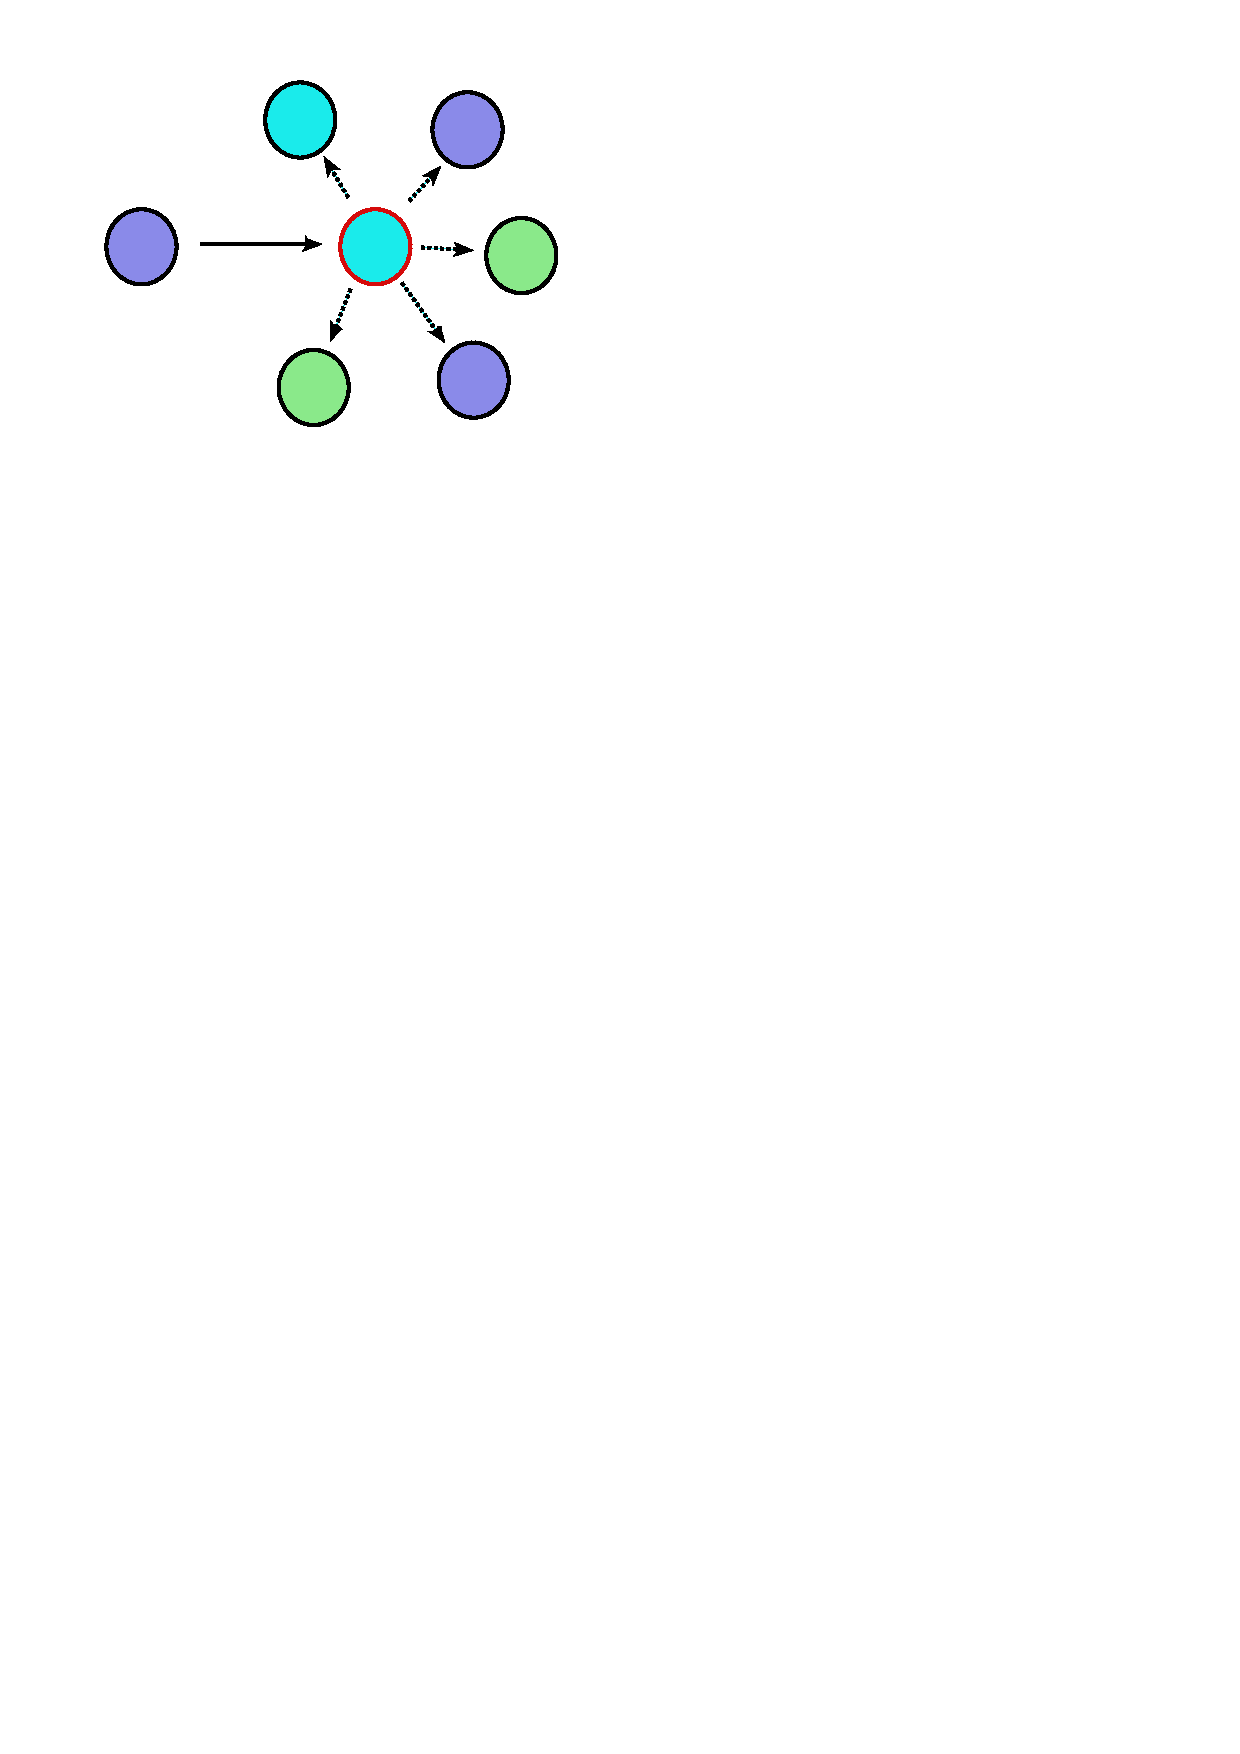
\includegraphics[width=\textwidth]{upstream.pdf}
            \caption{}\label{upstream}
        \end{subfigure}
        \qquad
        \begin{subfigure}[b]{0.4\textwidth}
		  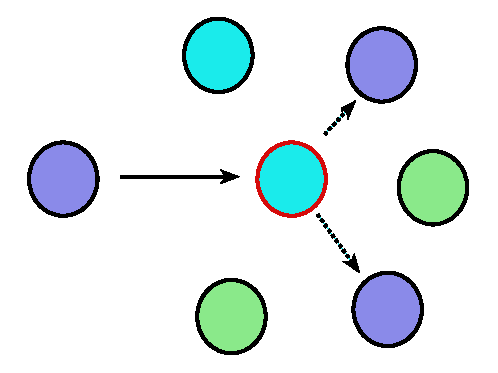
\includegraphics[width=\textwidth]{group.pdf}
            \caption{}\label{group}
        \end{subfigure}
        \caption{Upstream reciprocity. (\textit{a}) Someone who was helped or harmed becomes more likely to help or harm others. (\textit{b})
    Upstream group reciprocity targets people who belong to
    the same group as the initial partner.}
        \label{fig:illustration}
	\end{center}
\end{figure}

The concept of group reciprocity may help to explain the evolution of intergroup conflict. The current literature 
includes three differing approaches to understanding this. While cultural theories argue that there is no innate tendency to 
intergroup aggression, theories of parochial altruism argue that intergroup violence was a driver of within-group 
altruism via group selection processes; as a result, intergroup violence can involve self-sacrifice for one's group
members \citep{choi2007coevolution,bowles2009did}. ``The chimpanzee model", by contrast, argues that early humans, like
chimpanzees, only attack when odds are very favourable; thus a human tendency to kill outgroups evolved by individual
selection alone \citep{wrangham2012intergroup}. This is supported by evidence that both 
hunter-gatherers and chimpanzees are rarely wounded when they attack. A puzzle for the chimpanzee model, however, is 
that intergroup conflict among hunter-gatherers appears rare \citep{fry2013lethal}. 

We argue that group reciprocity can evolve in an environment where attacks are motivated by self interest, and provides 
a check for intergroup violence. Paradoxically, group reciprocity---while having the potential to expand the circle of 
violence---could explain the rarity of conflict among hunter-gather\-ers.
When there is group reciprocity, someone who harms an outgroup member brings retaliation on his own group. This gives 
his group members an incentive to maintain peace \citep{boehm1984blood}. By contrast, while 
chimpanzees do practice retaliation and reconciliation among alliances within the band, they  do not reciprocate towards 
other bands. Instead, they attack stranger chimpanzees whenever it is safe to do so. The risk of being attacked forces chimps
to avoid territory bordering other bands, which limits their available space for foraging \citep{wilson2003intergroup}.
\citet{kelly2005evolution} argues that this fact favours the evolution of peaceful intergroup relations, but this ignores
the prisoner's dilemma structure of intergroup relations; while both groups would
do better not attacking the other, each group does better by attacking when the odds are good enough.
By encouraging retaliation against attacks, the evolution of group reciprocity could solve this problem, and could thus
have benefited humans by allowing them to range over wider areas and to have more 
extensive contacts with outgroups. \citet{kelly2000warless} argues that group reciprocity (``social substitutability") is
more important when there is a strong political clan organization; however, hunter-gatherers do sometimes practice group 
reciprocity \citep{boehm2012ancestral}. Thus, modifying the chimpanzee model by adding group reciprocity may help to 
explain the relative peacefulness of hunter-gatherer bands. 

While group reciprocity can benefit the group, to evolve it must increase individual fitness. We suggest that this can
happen when the benefit/cost ratio of helping (or not harming) an outgroup member is high enough. The environment is the
following. Individuals are divided into groups of size $n$. In each period, each individual has an opportunity to help or
harm a randomly chosen outgroup member (the ``target"). Helping has a fitness cost~$c$ while providing a benefit~$b$ to 
the target (alternatively, $c$ can be viewed as the benefit to the actor from exploiting the interaction partner, thereby
imposing on them a harm of~$b$). Individual strategies are of two types: selfish or group reciprocal.
Selfish types never help, while group reciprocators help in their first interactions, and then help with a probability
proportional to the number of times they have been helped before by any member of the group of their current target. In the
supplementary materials, we report on a series of simulations tracking the evolution of group reciprocators under different
environmental parameters. We show that group reciprocity can evolve to fixation if $b/c$ is high enough relative to $n$; 
that is, the group benefit from maintaining a cooperative/peaceful reputation is a public good within the group. 

The mechanism is that groups with a high share of group reciprocators learn to cooperate with each other, while not helping
groups that have a high share of selfish types. Selfish types in cooperative groups free ride on the group reputation,
exploiting members of other cooperating groups, thereby gaining higher fitness then the group reciprocators in their group.
Nonetheless, if the share of group reciprocators within the group varies sufficiently between groups, group reciprocators 
are overrepresented in the cooperative groups, and therefore have higher fitness overall.
% removed this because I wasn't sure it helped understand the phenomenon.
% (this structure, where group
% reciprocators have higher fitness overall despite having lower fitness within each group, mirrors the well-known Simpson
% paradox).

The high $b/c$ ratio required for group reciprocity to evolve fits the ``chimpanzee model" of conflict where attacks are 
only launched if it is low risk. This may also explain why most salient examples of group reciprocity are seen in the
``negative" domain of harm and conflict. When $b/c$ is high, hurting or refraining from helping is a ``nasty" thing to 
do, since it imposes a large loss on the target for a small gain to oneself.

Thus, we hypothesise that humans developed a propensity to reciprocate towards groups. Although field observations from
conflict are highly suggestive, they are loaded with individual and group context and history. Moreover, in the natural 
world it is difficult to distinguish between retaliatory acts directed at groups that include the perpetrator and acts
directed at unrelated group members. We therefore designed a laboratory experiment to test the proximate mechanism implied
by our evolutionary model in a clean way. That is, we test the hypothesis that people reciprocate towards groups.

Cleanly identifying group reciprocity requires controlling for three confounds: individual level reciprocity, e.g. if
subjects' actions affect an entire group including the original actor who helped or harmed them; generalized reciprocity,
where subjects reciprocate not specifically towards the original actor’s group, but towards other people in general; and
strategic interactions, where apparent reciprocity is driven by reputation-building. 
our experiment fulfils all three: subjects can differentiate the original actor from his or her group members, they 
interact both with these group members and with members of other groups, and we minimize strategic concerns by not giving
feedback about subjects' actions.

%While previous work has not satisfied all three conditions simultaneously \citep{gaertner2008whenrejection,stenstrom2008theroles,hugh-jones2013intergroup}, 

While previous studies looked at retaliation towards groups, this retaliation does not necessarily reflect group reciprocity as defined here. \citet{gaertner2008whenrejection} found that rejection by one group member leads to more hostility towards the group when the group is perceived as a unified entity. Since hostility was directed towards the whole group, individual and group level reciprocity were confounded. Similarly, \citet{bohm2016makes} examine intergroup retaliation using the intergroup prisoner's
dilemma paradigm, but cannot distinguish between individual and group reciprocity.
\citet{stenstrom2008theroles} manipulated entitativity by making the original perpetrator (a political analyst) an official affiliate of the group (a presidential campaign). Thus, holding the group accountable for its member's action is justified without resorting to group reciprocity. In contrast, we look at how people reciprocate a clear individual act by one group member to an unrelated other group member, where group structure is minimal and free of existing social context. 


Our experimental set up was the following. After an initial group-formation stage, participants interacted in two strategic stages. The upstream action, in which the individual could be helped  or harmed by another person, was represented by a Trust Game (TG) \citep{berg1995trust}.  In this game, the Sender~(S) receives~150 money-equivalent tokens, and chooses how many of them to send to the Responder~(R). The amount sent is multiplied by a factor of~3, so that R receives between 0~and~450 tokens, of which he can send any number back to S. The TG enables us to model two types of interactions. Whereas R is clearly kind when returning money (and nasty when exploiting a generous proposer by keeping the received amount), S's intentions are equivocal. Sending money can be driven by selfish expectations of reciprocity, while not sending can be driven by caution. Thus, while all subjects experience helpful or harmful actions, only senders experience actions that clearly reflect their counterpart's preferences and intentions \citep{gunnthorsdottir2002using,kimbrough2015norms}.

The upstream action was followed by the reciprocal action, 
in which the individual could help others. We implemented this as an Allocation
Game in which subjects divided a fixed amount between two recipients.
In Direct Reciprocity rounds, the recipients included the TG partner;
in Group Reciprocity rounds, a member of the TG partner's group; and
in Ingroup Favoritism rounds, a member of the allocator's group.
The other recipient was always a member of a third, neutral, group.
Baseline rounds included two neutral recipients, to test whether the
TG experience leads to arbitrary discrimination in the absence of any reciprocal
or group motivations.

Our expectations were as follows. First, in Direct Reciprocity rounds, individuals' allocations to their TG partner
should positively covary with the amount the partner sent (or returned) in the Trust Game. This simply comes from
from the well-known theory of direct reciprocity. Second, if group reciprocity is present, then allocations to the TG partner's group member, in Group Reciprocity rounds, should also covary with the amount sent or returned by the TG partner.
We also measured participants' social value orientation \citep{van1999pursuit}. It is plausible that willingness to group-reciprocate should
be linked to other social preferences. We were not certain \emph{a priori} whether group reciprocity would be stronger
among selfish or among prosocial types. On the one hand, both prosociality and group reciprocity can be seen as actions
that benefit the group, by providing support to ingroup members or protecting it from outgroups. On the other hand,
negative reciprocity in general may be linked to spite \citep{johnstone2004evolution}. So we test a non-directional hypothesis here.

\section{Material and methods}
\label{sec:design}

Each session consisted of~24 participants, randomly allocated into six
\emph{teams} of four. Each participant was identified throughout the experiment
by team colour and individual number (1--4) within the team. At the beginning of
the experiment, participants were informed that the experiment had five distinct
stages, and that they might interact with the same people in different stages.
Specific instructions for each stage were distributed and read aloud at the
beginning of the stage. The five stages were a group formation stage, the TG
stage, the Allocation Game stage, a social value orientation elicitation stage
\citep*{murphy2011measuring} and a collectivism scale measurement stage
\citep*[adapted from the horizontal collectivism scale
in][]{Singelis1995horizontal}.

Following \citep{chen2009group}, we created group identity in the
first stage by allowing participants to consult each other by anonymous
chat while solving a simple task. Participants solved five Raven matrices
(see supplementary material). Each matrix was presented on screen
for 120~seconds, during which each participant could both send written
messages to the team and update her own answer. The final answer submitted
at the end of the 120~seconds determined payoffs, with 10~tokens
paid for each correct answer. To further boost group identity through
a common goal, team members each earned an additional bonus of 5~tokens
if all four team members answered correctly.

Next, participants were rematched into pairs to play the one-shot
TG. To facilitate understanding, participants played five practice
rounds, in which they entered decisions both as~S and as~R. In the
actual interaction, participants could see their TG partner's team
colour and individual number. 

The third stage Allocation Game consisted of six rounds. In each round, participants interacted
in groups of three. Individuals in each group were identified to each other by
team colour and number. Each round consisted of a random dictator game, as
follows. Each player in the group of three had to allocate 100~tokens within the
group. The allocator received a fixed 30~tokens, and could freely allocate the
remaining 70~tokens between the other two players. Previous research has found that
people do not harm, but refrain from helping negatively perceived outgroups
\citep{weisel2015ingroup}. Accordingly, we set the parameters of the game so
that, compared to the reference point of the allocator's own share, an equal
division benefits both other players. Table~\ref{tab:example} shows the matching scheme over the six rouds. Each participant was in the same group of three in one of the six rounds with a
member of her own team (\emph{ingroup} condition), in one round with her TG partner
(\emph{direct reciprocity} condition), and in two rounds with other members of the TG
partner's team (\emph{group reciprocity} condition). The remaining two rounds
served as the baseline condition. No feedback was provided between rounds. Stage payoffs were determined by one randomly chosen round of the six rounds, and
the allocation decision of one randomly chosen player in each group. Note that the matching is not independent. For example, if one player is in the direct reciprocity condition, then one other player
is in the direct reciprocity condition and the third player is in either the baseline or group
reciprocity condition. 

\begin{table}
  \caption{Matching example}\label{tab:example}
  \begin{center}
    \begin{tabular}{lcccc}
    \toprule
    Round	&	\multicolumn{3}{c}{Allocates to}		&	Treatment	\\
    \midrule
    1	&	\color{red}Red 1	&	/	&	\color{yellow!80!black}Yellow 1	&	Group reciprocity (GR)	\\
    2	&	\color{yellow!80!black}Yellow 4	&	/	&	\color{brown}Brown 2	&	Group reciprocity (GR)	\\
    3	&	\color{green!60!black}Green 3	&	/	&	\color{yellow!80!black}Yellow 2	&	Direct reciprocity (DR)	\\
    4	&	\color{red}Red 1	&	/	&	\color{brown}Brown 1	&	Baseline (B)	\\
    5	&	\color{brown}Brown 2	&	/	&	\color{brown}Brown 4	&	Baseline (B)	\\
    6	&	\color{blue}Blue 3	&	/	&	\color{green!60!black}Green 2	&	Ingroup (IG)	\\
    \bottomrule
    \multicolumn{5}{p{0.7\textwidth}}{\footnotesize
	Note: Example treatments shown for player {\color{blue}Blue 2}, who played the TG with {\color{yellow!80!black}Yellow 2} (see the supplementary material for the full matching scheme).    
    }
    \end{tabular}
  \end{center}
\end{table}

The fourth stage implemented the slider measure of social value orientation
\citep*{murphy2011measuring,crosetto2012flexible}, in which participants
choose nine allocations between themselves and another person. For
consistency with the previous stages, the team identity of the partner
was known. To keep the decision independent of previous experience
with the different teams, we matched participants within teams. Therefore, this measure captures within-group social value orientation. Payoffs
were determined by one randomly chosen decision of the nine decisions
made by one randomly chosen player in each dyad. The decisions yielded
a social orientation angle for each participant, with~$0^{\circ}$
corresponding to selfishness, $45^{\circ}$ to pure altruism, and
negative angles to spitefulness.

After the fifth and final stage (a non-strategic and non-incentivised
collectivism measurement), participants learned their cumulative payoff in tokens and were paid in private.
%and final payment in New Israeli Shekels. 
One hundred and ninety two participants, recruited using ORSEE \citep*{greiner2015subject} participated in eight sessions conducted between June 2014 and January
2015. %Due to software malfunction in one session, the data from the AG sixth round were not saved. 
The experiment was programmed in z-Tree
\citep*{Fischbacher2007}. 
%The average payment was 72~NIS (approximately \$18) for a duration of 70~minutes

The key outcomes in this design are based on the allocation decisions made in the third stage. Direct and group reciprocity can be both positive and negative, and therefore are not hypothesized to have a systematic effect on the the amount allocated to either the TG partner or to his team mates. Nonetheless---while there is arguably no reason to discriminate between two neutral players---we hypothesize that direct and group reciprocity will lead the allocator to discriminate either for or against the TG partner or his team mates. Consequently, we predict that the absolute difference between the two allocations will be larger in all treatments compared to the baseline. This difference is measured in our `Discrimination' outcome.

We measure reciprocity directly by looking at the effect of the TG experience in the second stage on allocations made in the third stage. We define the experience with the TG partner in two ways. For responders, this is the amount sent to them by their partner. For senders, we calculate the amount returned to them by their partner as a fraction of the money available to the responder. Thus, an equal split of the pie implies a value of 1/2, and compensating the sender for his investment implies a value of 1/3. We subsequently define (direct or group) reciprocity as the slope of the allocation made to the TG partner or his team mates on the TG experience.

\section{Results}
\label{sec:results}

We report results on allocations, discrimination between recipients (measured as the
absolute difference between the two recipients' allocations), and direct and
group reciprocity. All reported statistical tests are based on mixed-effects
regressions with bootstrapped standard errors clustered on subjects. %See the supplementary material for the full specification and results.


\begin{kframe}


{\ttfamily\noindent\color{warningcolor}{\#\# Warning in sqrt(diag(se)): NaNs produced}}\end{kframe}%latex.default(tbl[, -1], file = "", label = "tab:results", rgroup = c("Senders",     "Responders"), caption = "Allocations and Discrimination",     rowname = tbl$Condition, center = "centerline", rowlabel = "",     insert.bottom = "\\justify Mean allocation, mean discrimination, and reciprocity (marginal effect of TG partner's kindness on allocation) by condition. Robust standard errors clustered on sessions. Significance of comparison to Baseline is marked.$^{*}$, $^{**}$, and $^{***}$ indicate p $<$ 0.05, p $<$ 0.01, and p $<$ 0.001, respectively.")%
\begin{table}[!tbp]
\caption{Allocations and Discrimination\label{tab:results}} 
\centerline{\begin{tabular}{llll}
\hline\hline
\multicolumn{1}{l}{}&\multicolumn{1}{c}{Allocation}&\multicolumn{1}{c}{Discrimination}&\multicolumn{1}{c}{Reciprocity}\tabularnewline
\hline
{\bfseries Senders}&&&\tabularnewline
~~Baseline&35.00 (---)& 4.15 (1.13) &---\tabularnewline
~~Direct Reciprocity&33.98 (2.30) &22.00 (1.51) ***&15.64 (5.12)**\tabularnewline
~~Group Reciprocity&34.39 (0.77) & 8.08 (1.61) ***& 7.78 (2.37)**\tabularnewline
~~In-Group&38.98 (1.11) ***&15.46 (2.99) ***& 0.20 (5.50)\tabularnewline
\hline
{\bfseries Responders}&&&\tabularnewline
~~Baseline&35.00 (---)& 2.25 (0.51) &---\tabularnewline
~~Direct Reciprocity&35.38 (1.08) &22.17 (2.30) ***&20.87 (6.04)***\tabularnewline
~~Group Reciprocity&34.79 (0.62) & 6.12 (1.51) **& 1.20 (2.08)\tabularnewline
~~In-Group&42.13 (1.99) ***&17.20 (3.40) ***& 4.72 (7.62)\tabularnewline
\hline
\end{tabular}}
\justify Mean allocation, mean discrimination, and reciprocity (marginal effect of TG partner's kindness on allocation) by condition. Robust standard errors clustered on sessions. Significance of comparison to Baseline is marked.$^{*}$, $^{**}$, and $^{***}$ indicate p $<$ 0.05, p $<$ 0.01, and p $<$ 0.001, respectively.\end{table}



The first column in Table~\ref{tab:results} presents the mean allocations.
Participants gave significantly more to members of their own team at the expense
of the neutral recipient ($z=3.58,p< 0.001$ for senders, 
$z=3.59,p< 0.001$ for
responders), establishing that our group formation manipulation was successful
in inducing group identity and triggering ingroup favouritism. Allocations to
the TG~partner and his team mates were not significantly different to the
baseline~35 ($p>0.43$ for all comparisons). This result suggests that the experience with the TG partner is, on average, neutral, such that positive and negative experiences balance each other overall.

Nonetheless, both positive and negative treatment of the TG partner or his team mates increase the absolute difference between the two allocationa. Indeed,
column of Table~\ref{tab:results} shows that allocators discriminated significantly more
than in the baseline both when interacting with their TG partner
($z=9.08,p< 0.001$) and with his team mates 
($z=3.93,p< 0.001$). This effect was not
significantly different between TG senders and receivers (F test $0.50,
p= 0.68$).

\subsection{Direct and group reciprocity}
\label{sec:reciprocity}

The third column of Table~\ref{tab:results}, \emph{Reciprocity}, reports the slope of
allocations regressed on the subjects' experience with their TG partners. 
The responder's experience with the sender is measured
as the share of the endowment that the sender chose to send. The sender's experience with the responder is measured as the share
of the received amount that the responder chose to send back. 
The sender's experience was not defined
for the six (out of 96) senders who did not send any money.
%
There is strong direct reciprocity: allocations
to the TG partners increase with the TG experience both for
senders ($z=3.06,p< 0.01$) and for responders 
($z=3.46,p< 0.001$).

Group reciprocity, however, is only observed for senders, who allocate
less to team mates of a responder who returned less---an intentionally harmful action.
Responders, on the other hand, although directly reciprocating the
TG partner's action, do not systematically discriminate against team mates
of a sender who sent little---a harmful action that does not unequivocally
signal a bad intention. The regression analysis shows no significant
effect of the responder's TG experience on her allocation to the sender's
team mates ($z=0.58,p= 0.56$). 
The sender's TG experience, on the other
hand, significantly increases the allocations made to the responder's team mates 
($z=3.29,p< 0.01$).
The estimated ratio of the group and direct reciprocity coefficients
is 50\%, so that for every allocation dollar a responder
loses due to an unkind action in the TG, his team mates lose~50 cents. 
This relationship is presented graphically in Figure~\ref{fig:plots} (the corresponding figure for direct reciprocity is included in the supplementary material).



% The median kindness of responders was $\frac{1}{3}$, which compensates senders
% exactly for the amount they sent. To compare the strength of ``positive'' and
% ``negative'' group reciprocity, we split senders by whether their TG partners
% sent less than $\frac{1}{3}$, exactly $\frac{1}{3}$ or more than $\frac{1}{3}$. The mean allocations in the
% group reciprocity condition for these three groups were give_ks3[1], give_ks3[2] and give_ks3[3]
% respectively. Those whose partners sent less than $\frac{1}{3}$ allocated significantly
% less than the other two groups (Mann-Whitney test at individual level, ), which were not significantly
% different from each other (XXX t test). Thus, behaviour is driven by negative
% group reciprocity. This accords with real world evidence: reports of negative
% reciprocity are much more widespread than for positive reciprocity.

Senders' group reciprocity was related to their social value orientation. The slope of the effect of the TG experience on allocations was 
15.97 for those with less than median SVO, and 
-1.06 for those with median or greater SVO 
(interaction, $p= 0.061$).These results should be interpreted cautiously, since both scores were 
affected by the TG experience. 

\begin{knitrout}
\definecolor{shadecolor}{rgb}{0.969, 0.969, 0.969}\color{fgcolor}\begin{figure}
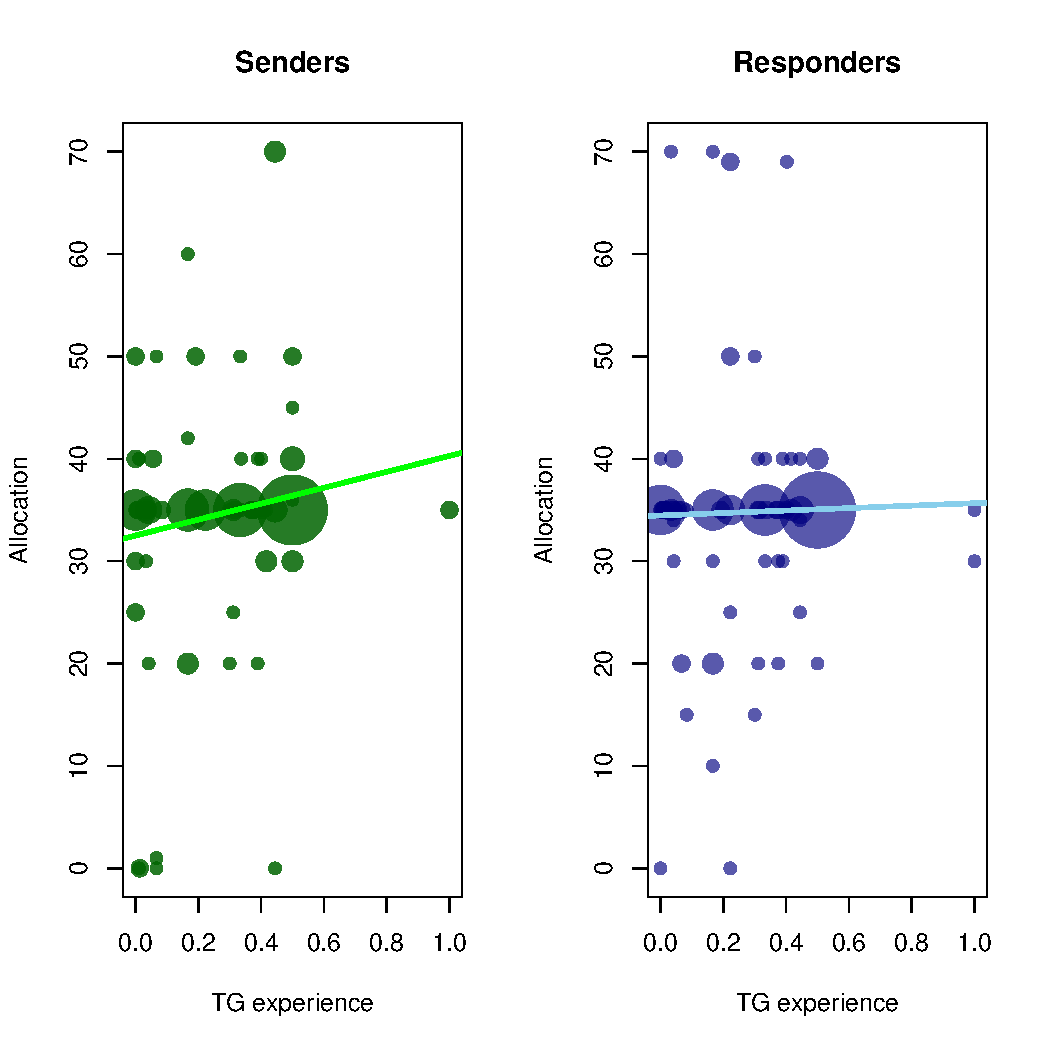
\includegraphics[width=\maxwidth]{figure/plots-1} \caption[Allocations in the Group Reciprocity condition versus the TG experience]{Allocations in the Group Reciprocity condition versus the TG experience. Circles show individual data points (circle size proportional to number of observations). Lines show linear regressions.}\label{fig:plots}
\end{figure}


\end{knitrout}

\section{Discussion}
\label{sec:conclusion}

Our results show that upstream reciprocity is moderated by social boundaries. 
Humans respond to harms from outgroup members by discriminating against others 
in that specific outgroup. This supports the argument of \citet{Pietraszewski2016470} that group identity can modify the cost-benefit calculus of individuals deciding whether to extend a conflict. 

We distinguish between reciprocity towards harm and towards intentional harm
\citep{stanca2009testing}. People discriminate against others who harm them even
if the harmful action does not necessarily indicate bad intentions. However,
they only generalize to the perpetrator's  group members if the intentions
behind the harmful actions are unequivocally bad.

This observation raises new questions regarding the nature of reciprocity
and the role of intentions (or perceptions thereof). One possible
interpretation stems from the distinction between intention-based
and outcome-based motives in reciprocal behaviour \citep{falk2006theory}. It is
possible that humans generalize intentions across group members more than they generalize
actions across group members. So, if (e.g.)  group member 1 wishes to harm them,  they are prone to infer
that group member 2 also wishes to do so; but if group member 1 takes an action
that harms them, they do not necessarily infer that group member 2 would also
have done so. Indeed, the conjecture `One member of the Blue
group is a bad person, therefore all Blue members are bad' is plausible.
The conjecture `One member of the Blue group did not send any money,
therefore other Blue members did not send money' is not---as, given subjects' knowledge, the other Blue members may not even had the opportunity to send any money.

One caveat is in order.
% deals with point 5
Since our study was conducted with students from a rich industrialized democracy, results may not generalize to all cultures \citep{henrich2010most}. In particular, the link between intentions and moral judgment may vary across cultures \citep{barrett2016small}, and this could affect how group reciprocity plays out in different societies.

Group reciprocity as a proximate mechanism bears implications for human social cognition. While ingroup altruism and group-based downstream reciprocity require people to differentiate their own group from outsiders ---``us'' from ``them''---upstream group  reciprocity requires them to differentiate between different outgroups---between ``them and them''---and to keep a mental account of outgroups' reputation. Thus, group reciprocity could provide a cognitive foundation for the phenomena of intergroup prejudice and stereotyping \citep{allport1954nature}.



% new para, not sure quite where to put it
We have argued that group reciprocity could help explain hunter-gatherers' relatively peaceful intergroup relations. It may
also provide a step from the ``chimpanzee model" of conflict towards the large-scale, organized intergroup conflicts
observed in tribal and state-level societies. A further step could be provided by ``third party" group reciprocity. That 
is, in many ethnic conflicts, a harm from one group to another is revenged by the entire second group, leading to 
cycles of intergroup violence. Third party group reciprocity could result from organized groups taking collective
action to maintain their reputation as reciprocal (and hence, dangerous to attack).

Upstream reciprocity is notoriously difficult to understand in evolutionary
terms \citep{boyd1989evolution,nowak2007upstream}. Group reciprocity
may provide another piece of the puzzle, as it allows upstream reciprocity to direct group-level selection in ways parallel 
to those by which direct reciprocity direct individual-level selection.
%provides two new channels by which upstream reciprocity may evolve. 
We acknowledge, though do not develop here, two other ways by which group reciprocity may evolve.
First, group members are interdependent, especially in the small groups that were the norm during most of human evolutionary 
history. Punishing a perpetrator's group member therefore indirectly harms the perpetrator, who is dependent on his peers for
, e.g., public goods provision. Thus, group reciprocity may bridge upstream indirect reciprocity and direct reciprocity 
through intra-group dependencies. Second, the evolution of indirect reciprocity acts by way of chains
of reciprocal actions, which return with some probability to the original
instigator of the chain \citep{nowak2007upstream}. In a population
organised in groups, such that individuals interact more frequently with
their own group members, group reciprocity may increase the likelihood
of successful reciprocal chains, facilitating the evolution of upstream
reciprocity. These ideas could be formalized in future work.

%\section*{Acknowledgements}
%This research was supported by the ISRAEL SCIENCE FOUNDATION (grant No. 214/13).


\newpage
\printbibliography
%\bibliographystyle{dcu}
%\bibliography{grouprec}

\newpage

\section*{\textsc{Supplementary materials}}

\setcounter{figure}{0}
\setcounter{section}{0}
\renewcommand\thesection{Appendix~\Alph{section}:}
\renewcommand\thefigure{\Alph{section}.\arabic{figure}}  

\section{Simulations}

We ran simulations of the evolution of group reciprocity as follows. The population consisted of $G$ groups of size $n$.
Each generation consisted of $T$ rounds. In each round, all individuals were matched with a randomly selected target 
from a different group. The individual could either help the target, losing $c = 1$ and benefiting the target $b$, or not 
help, which did not affect payoffs. 

Individuals were of two types. Selfish types never help. Group reciprocal types condition on their current target's group.
If they have never been targeted by someone from that group before, they help. If they have been targeted in the
previous $m$ rounds by one or more persons from that group, then they help with probability equal to the proportion of
times they were helped. For example, if they were targeted by persons from that group 5 times in the previous $m$ rounds,
and were helped 3 times, then they help with probability 3/5 = 60\%.

After each generation, each individual changed type with independently drawn probability $\pi = 0.05$, copying a 
new type from one other individual in the population. Individuals' probability of being copied was proportional 
to their own total payoff. This could represent either a process of success-biased cultural transmission, or evolution
with payoffs representing fitness and full mixing across populations. The simulation ran until one strategy evolved 
to fixation in the whole population.

Our base simulation has $T = m = 60$ and $G = 10$ groups, with the initial type distribution being 50\% selfish and
50\% group reciprocal, drawn independently for all individuals. We vary the benefit of being helped $b$, and the 
group size $n$, from 12 to 30. In the ``short memory" variant we set $T = m = 30$. In the ``many groups" variant 
we set $G = 20$. We ran ten simulations of each parameter configuration. Figure \ref{fig:simulations} shows the proportion of times that GR evolved to fixation. In each case, larger $b$ and smaller $n$ make it easier for
group reciprocity to evolve.




The mechanism for group reciprocity's evolution is as follows. The cost of helping is balanced against the benefit
that a target who is a group reciprocator will subsequently help one's own group with increased probability. In this
case, with probability $1/n$, one will oneself be helped. Thus, group reciprocity can evolve much like individual
reciprocity so long as the benefit/cost ratio $b$ is high enough. 


It is only advantageous to help if the target is a group reciprocator. Group reciprocity itself achieves this by
counting the number of times that help has come from the group. If there is sufficient variation between groups in the
proportion of group reciprocators, then this will be an effective heuristic, and groups with a good reputation will be
helped more. In the simulations, the correlation between
individual fitness, and the reputation of the individual's group (average number of times it had helped), was a good
predictor of whether GR would evolve to fixation: the mean correlation was 0.84 when GR fixed and 0.55 when selfishness fixed (p < 0.001).


\begin{figure}
	\begin{center}
		  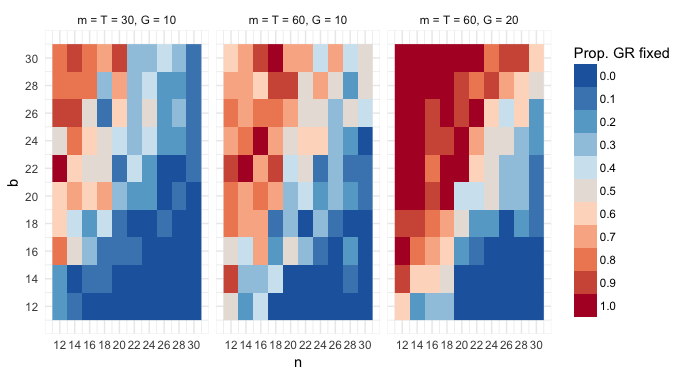
\includegraphics[width=\textwidth]{b-vs-gsize-all-sims.png}
        \caption{Simulation results. $b$ = benefit of being helped. $n$ = group size.}
        \label{fig:simulations}
	\end{center}
\end{figure}


\section{Complete matching scheme}
\begin{center}
\begin{sideways}\resizebox{0.9\textheight}{!}{

%\documentclass[12pt,a4paper]{article}
%\usepackage{multirow,rotating,booktabs}
%\usepackage{tabularx}

%\begin{document}

%\section*{Appendix A: Complete matching scheme}

%\begin{sidewaystable}[H]\footnotesize
%	\caption{Complete matching scheme}
%\begin{center}
%\begin{sideways}\resizebox{0.9\textheight}{!}{
\begin{tabular}{lc*{8}c}
  \toprule
  \multirow{3}{*}{Period}	&	&	\multicolumn{8}{c}{Group}	\\
  \cmidrule{3-10}
  	&	&	1	&	2	&	3	&	4	&	5	&	6	&	7	&	8	\\
  	\midrule
	\multirow{3}{*}{1}	&	&	Blue	2	(GR)	&	Blue 1 (GR)	&	Green 4 (GR)	&	Blue 3 (B)		&	Red 2 (DR)	&	Blue 4 (B)		&	Green 1 (IG)	&	Red 4 (B)	\\
		&	&	Red 1 (B)	&	Yellow 2 (GR)	&	Brown 4 (B)	&	Green 3 (GR)	&	Brown 2 (DR)	&	Red 3 (DR)	&	Green 2 (IG)	&	Yellow 3 (IG)	\\
		&	&	Yellow 1 (GR)	&	Purple 2 (B)	&	Purple 3 (GR)	&	Purple 4 (GR)	&	Purple 1 (B)	&	Brown 3 (DR)	&	Brown 1 (B)	&	Yellow 4 (IG)	\\
	\midrule
	\multirow{3}{*}{2}	&	&	Green 3 (GR)	&	Red 3 (B)	&	Blue 4 (GR)	&	Blue 2 (GR)	&	Blue 3 (DR)	&	Green 2 (DR)	&	Blue 1 (B)		&	Red 2 (IG)	\\
	&	&	Yellow 1 (B)	&	Green 1 (GR)	&	Green 4 (B)	&	Yellow 4 (GR)	&	Red 1 (B)	&	Brown 4 (B)	&	Brown 1 (IG)	&	Red 4 (IG)	\\
	&	&	Purple 1 (GR)	&	Purple 3 (GR)	&	Yellow 2 (GR)	&	Brown 2 (B)	&	Yellow 3 (DR)	&	Purple 2 (DR)	&	Brown 3 (IG)	&	Purple 4 (B)	\\
	\midrule
	\multirow{3}{*}{3}	&	&	Red 1 (GR)	&	Red 4 (GR)	&	Blue 3 (B)		&	Red 3 (GR)	&	Green 4 (DR)	&	Blue 2 (DR)	&	Blue 1 (IG)	&	Yellow 3 (B)	\\
	&	&	Brown 4 (GR)	&	Yellow 4 (B)	&	Red 2 (GR)	&	Green 2 (B)	&	Yellow 1 (B)	&	Green 3 (B)	&	Blue 4 (IG)	&	Purple 2 (IG)	\\
	&	&	Purple 1 (B)	&	Brown 1 (GR)	&	Brown 3 (GR)	&	Brown 2 (GR)	&	Purple 4 (DR)	&	Yellow 2 (DR)	&	Green 1 (B)	&	Purple 3 (IG)	\\
	\midrule
	\multirow{3}{*}{4}	&	&	Blue 4 (GR)	&	Blue 3 (GR)	&	Green 2 (GR)	&	Blue 1 (B)		&	Red 4 (DR)	&	Blue 2 (B)		&	Green 3 (IG)	&	Red 2 (B)	\\
	&	&	Red 3 (B)	&	Yellow 4 (GR)	&	Brown 2 (B)	&	Green 1 (GR)	&	Brown 4 (DR)	&	Red 1 (DR)	&	Green 4 (IG)	&	Yellow 1 (IG)	\\
	&	&	Yellow 3 (GR)	&	Purple 4 (B)	&	Purple 1 (GR)	&	Purple 2 (GR)	&	Purple 3 (B)	&	Brown 1 (DR)	&	Brown 3 (B)	&	Yellow 2 (IG) \\
	\midrule
	\multirow{3}{*}{5}	&	&	Green 4 (GR)	&	Red 4 (B)	&	Blue 3 (GR)	&	Blue 1 (GR)	&	Blue 4 (DR)	&	Green 1 (DR)	&	Blue 2 (B)		&	Red 1 (IG)	\\
	&	&	Yellow 2 (B)	&	Green 2 (GR)	&	Green 3 (B)	&	Yellow 3 (GR)	&	Red 2 (B)	&	Brown 3 (B)	&	Brown 2 (IG)	&	Red 3 (IG)	\\
	&	&	Purple 2 (GR)	&	Purple 4 (GR)	&	Yellow 1 (GR)	&	Brown 1 (B)	&	Yellow 4 (DR)	&	Purple 1 (DR)	&	Brown 4 (IG)	&	Purple 3 (B)	\\
	\midrule
	\multirow{3}{*}{6}
	&	&	Red 2 (GR)	&	Red 3 (GR)	&	Blue 4 (B)		&	Red 4 (GR)	&	Green 3 (DR)	&	Blue 1 (DR)	&	Blue 2 (IG)	&	Yellow 4 (B)	\\
	&	&	Brown 3 (GR)	&	Yellow 3 (B)	&	Red 1 (GR)	&	Green 1 (B)	&	Yellow 2 (B)	&	Green 4 (B)	&	Blue 3 (IG)	&	Purple 1 (IG)	\\
	&	&	Purple 2 (B)	&	Brown 2 (GR)	&	Brown 4 (GR)	&	Brown 1 (GR)	&	Purple 3 (DR)	&	Yellow 1 (DR)	&	Green 2 (B)	&	Purple 4 (IG)	\\
	\bottomrule
\end{tabular}
%}
%\end{sideways}
%\end{center}
%\end{sidewaystable}


%\end{document}

}
\end{sideways}
\end{center}

\newpage
\section{Allocations in the DR condition}

\begin{knitrout}
\definecolor{shadecolor}{rgb}{0.969, 0.969, 0.969}\color{fgcolor}\begin{figure}[!h]
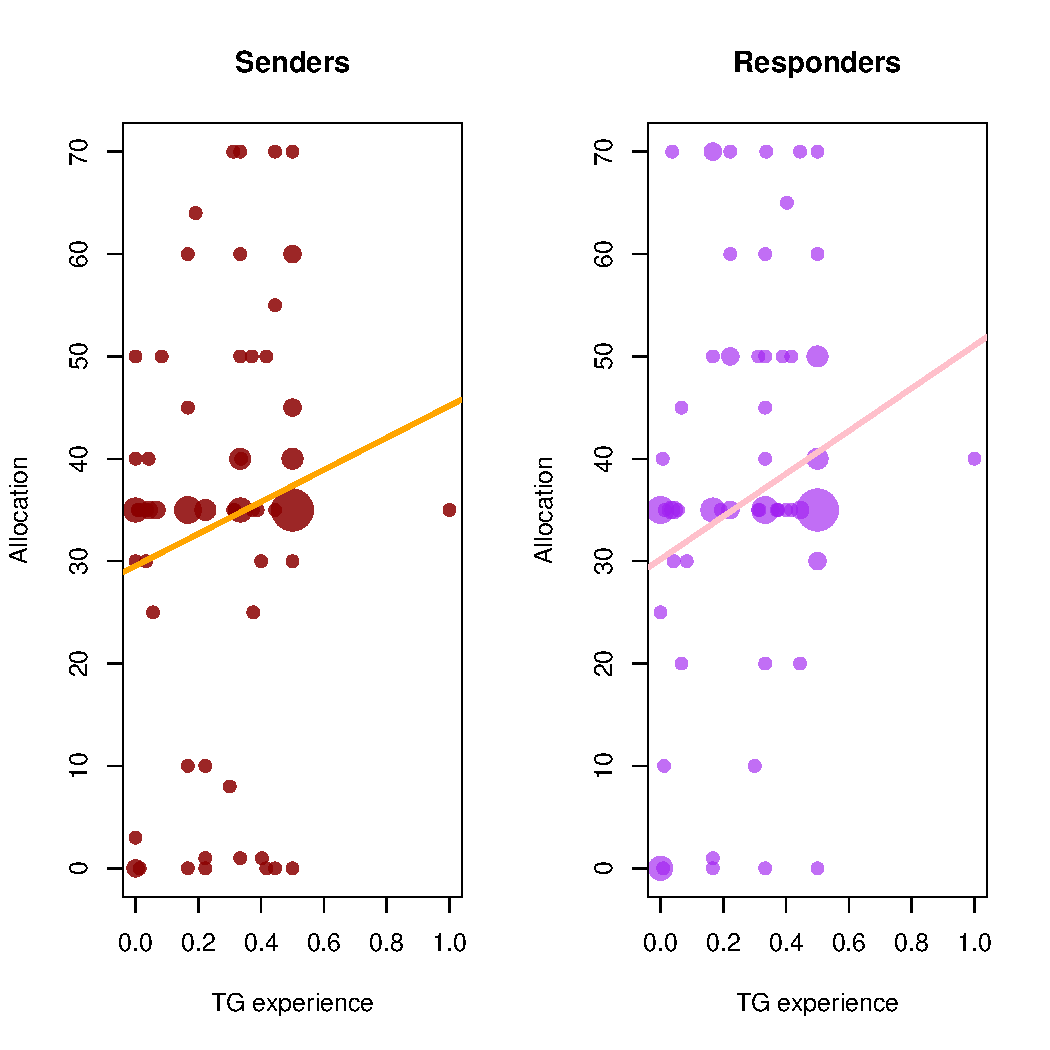
\includegraphics[width=\maxwidth]{figure/plots_dr-1} \caption[Allocations in the Direct Reciprocity condition versus the TG experience]{Allocations in the Direct Reciprocity condition versus the TG experience. Circles show individual data points (circle size proportional to number of observations). Lines show linear regressions.}\label{fig:plots_dr}
\end{figure}


\end{knitrout}

\newpage
\section{Experimental instructions}

%\documentclass[12pt,a4paper]{article}
%\usepackage{amsmath,amssymb,amsthm}
%\usepackage{geometry}

%\usepackage{changepage}

%\usepackage{xltxtra,fontspec,xunicode}
%\defaultfontfeatures{Scale=MatchLowercase,Mapping=tex-text}

%\usepackage{parskip}

%\begin{document}
\setlength\parindent{0pt}

%\section*{Appendix B: Experimental instructions}



\subsection*{Instructions for the experiment}
\emph{<Presented as a pdf document and available throughout the experiment>}
\bigskip

\textbf{These instructions are identical to all the participants.}

\textbf{The experiment is composed of five separate and different phases.} At the beginning of the experiment, all participants will be allocated into \textbf{teams of four}. Each team has a unique \textbf{colour}. These teams will remain fixed throughout the experiment.

Before each part, we will distribute and read the relevant instructions for that part. In each part the participants will be reallocated into groups. The number of participants in a group can change from part to part. The payments in the part will be determined according to the decisions of the participants in the team. It is possible, but not necessary, that another participant will be in the same group as you in two different parts. In each part of the experiment you will be able to know which team each of the participants in your group belongs to.

\textbf{Your final payment in the experiment will be the total of your gain in all of the parts}.

At the end of the experiment, you will be presented with the payments in each part and your total payment, in points and in shekels. Please remain seated until the experimenter calls you for payment.

\textbf{If you have any questions, please raise your hand now and the experimenter will come to you}.

\newpage

\subsection*{Experiments for the first part}

In this part, you and the members of your team perform a pattern completion task. The computer will present you with five questions. Each question is comprised of eight pictures, and the team members wil be asked to choose a ninth picture out of eight possible pictures to complete the pattern. For example:

\begin{center}
	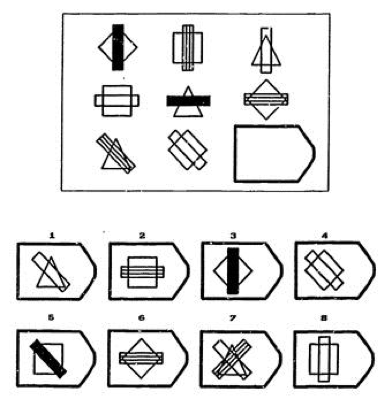
\includegraphics[]{Raven.png}
\end{center}

Each team member must answer all of the questions. For each correct answer, the team member will receive \textbf{10 points}. Additionally, if all of the team members answer correctly, the whole team will receive a \textbf{team bonus of 20 points, to be equally divided among the team members}.

\textbf{Each question will be allocated two minutes}. During this time, the team members can \textbf{consult each other} using electronic chat. Enter your answer and click Confirm. You can change your answer and click Confirm again at any point during the two minutes. The last answer to be entered is the final answer.

\textbf{Attention:} Do not reveal any identifying information. If any participant in the session identifies themselves, we will stop the experiment and release all participants with only the showup fee.

\textbf{If you have any questions, please raise your hand now and the experimenter will come to you}.

\newpage

\subsection*{Instructions for the second part}

In this part participants will be matched in \textbf{pairs}. In each pair, one participant will be in role A and the other participant in role B. Participant A receives an allocation of \textbf{150 points} and decides how many of the 150 points to \textbf{send to Participant B}. The amount is \textbf{tripled}. Next, Participant B will decide how many points out of the points received to \textbf{send back to to Participant A}. These points will not be multiplied.

If you are allocated to role A, your payment in this part will be:

\newcommand{\boxit}[2]{\fbox{\begin{minipage}[c][4cm][c]{#1}\centering #2\end{minipage}}}
\setlength\fboxrule{3pt}

{\medskip%\hspace{-2cm}
\begin{adjustwidth}{-0.6in}{-0.6in}
\large
\sffamily\centering
\boxit{1.5cm}{\Huge 150} -
\boxit{4cm}{The number of points you sent to Participant B} +
\boxit{4cm}{\large The number of points Participant B sent back} =
\boxit{2cm}{Second part earnings}
\end{adjustwidth}
}\medskip

If you are allocated to role B, your payment in this part will be:

{\medskip%\hspace{-2cm}
\begin{adjustwidth}{-0.6in}{-0.6in}
\large
\sffamily\centering
\boxit{1.5cm}{\Huge 3} $\times$
\boxit{4cm}{The number of points Participant A sent you} -
\boxit{4cm}{\large The number of points you sent back} =
\boxit{2cm}{Second part earnings}
\end{adjustwidth}
}\medskip

Before making your decision, you will be able to test the payment calculation in a \textbf{practice phase}, in which you will be able to make decisions as both \textbf{Participant A} and as \textbf{Participant B}. In this stage, you will enter decisions in both roles, and see the final payments. The practice will repeat five times. 

\textbf{If you have any questions, please raise your hand now and the experimenter will come to you}.

\newpage

\subsection*{Instructions for the third part}

In the third part, all participants will be matched in \textbf{groups of three}. Each of the three participants in the group will choose how to \textbf{divide 100 points} between the three group members, such that he himself receives \textbf{30 points}, and \textbf{freely allocates} the remaining \textbf{70 points} between the other two group members. This stage has \textbf{6 rounds}, and you will be \textbf{rematched in a new group}.

\subsection*{Payment calculation in the part}

At the end of the experiment, the computer will randomly choose one of the six rounds, and one participant in each group. The payment for this part will be determined according to the decision of the randomly chosen participant in the randomly chosen round.

\textbf{If you have any questions, please raise your hand now and the experimenter will come to you}.

\newpage

\subsection*{Instructions for the fourth part}

In this part, participant will be matched in \textbf{pairs}. 

Each participant will be presented with \textbf{6 rulers} that include nine possible allocations of money to the two participants. The amount you chose to \textbf{keep for yourself} is indicated above each ruler, and the amount you choose to \textbf{give to the other participant} is indicated below the ruler. You are to choose your preferred allocation of the nine possible allocations. For example, 
\smallskip

\begin{center}
	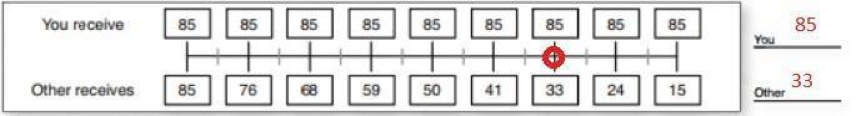
\includegraphics[]{svo.png}
\end{center}

You can choose any point on the ruler. For example, assume you chose the point marked in red. You will receive 85 points and the other participant will receive 33 points.

At the end of the part, the computer will randomly choose on of the two participants in the pair and one of the nine rulers. your payment in this part will be determined by the decision of the randomly chosen participant for the randomly chosen ruler.

\textbf{If you have any questions, please raise your hand now and the experimenter will come to you}.

\newpage

\subsection*{Instructions for the fifth part}

In this part you will be asked to answer several questions. The questions have to do with the way one sees himself and his surroundings in different situations. Your task is to indicate how much you agree or disagree with each statement, using the following scale:
\begin{enumerate}
	\item Strongly disagree.
	\item Disagree.
	\item Neither agree nor disagree.
	\item Agree.
	\item Strongly agree.
\end{enumerate}

Note: there are no right and wrong answers. Please indicate the answer that best reflects your character with respect to the statement. Take your time and think about your answer.


%\end{document} 

\end{document}
